\documentclass[compress]{beamer}
\mode<presentation>
{
 \usetheme{Vilanova}
}

\usepackage[english]{babel}

\usepackage[utf8]{inputenc}

\usepackage{times}
\usepackage[T1]{fontenc}

\usepackage{amsfonts}
\usepackage{amsmath}
\usepackage{amssymb}
\usepackage{tikz}
%\usepackage{url}
\usepackage{verbatim}


\title{Image radiometry in ORFEO Toolbox}

\subtitle
{From digital number to reflectance} % (optional)


\author
{J. Inglada\inst{1} , E. Christophe\inst{2}}
\normalsize

\institute[Cesbio, Crisp] % (optional, but mostly needed)
{\inst{1}\textsc{Centre d'Études Spatiales de la Biosphère, Toulouse, France}
\and
\inst{2}\textsc{Centre for Remote Imaging, Sensing and Processing,\\ National University of Singapore}
}

\date{}

\pgfdeclareimage[height=96mm,width=128mm]{background}{fondsClairSansLogo}
\setbeamertemplate{background}{\pgfuseimage{background}}
\pgfdeclareimage[height=0.6cm]{logoIncrust}{logoIncrust}
\pgfdeclareimage[height=0.5cm]{logo_cesbio}{logo_cesbio}
\pgfdeclareimage[height=0.35cm]{logo_crisp}{logo_crisp}
\logo{
\begin{tabular}{lp{0.10\textwidth}lp{0.25\textwidth}r}
\href{http://www.cesbio.ups-tlse.fr/}{\pgfuseimage{logo_cesbio}}\href{http://www.crisp.nus.edu.sg/}{\pgfuseimage{logo_crisp}}
&&\footnotesize{IGARSS 2010, Honolulu}&&
\href{http://www.orfeo-toolbox.org}{\pgfuseimage{logoIncrust}}\\
\end{tabular}
}


\subject{Image radiometry in ORFEO Toolbox}

% Delete this, if you do not want the table of contents to pop up at
% the beginning of each subsection:
\AtBeginSubsection[]
{
  \begin{frame}<beamer>
    \frametitle{Outline}
    \tableofcontents[currentsection,currentsubsection]
  \end{frame}
}




% If you wish to uncover everything in a step-wise fashion, uncomment
% the following command: 

% \beamerdefaultoverlayspecification{<+->}

\begin{document}

\begin{frame}
  \titlepage
{\tiny This content is provided under a Creative Commons
  Attribution 3.0 Unported License} \href{http://creativecommons.org/licenses/by/3.0/}{\includegraphics[width=0.05\textwidth]{../Ressources/CC-licence.png}}
\end{frame}

\section*{Introduction}

\begin{frame}

  \frametitle{Introduction}
  \begin{block}{Purpose of radiometry}
   \begin{itemize}
   \item Go back to the physics from the image
   \end{itemize}
  \end{block}
  \begin{block}{6S}
   \begin{itemize}
    \item Using 6S library: http://6s.ltdri.org/
    \item Library heavily tested and validated by the community
    \item Translation from the Fortran code to C
    \item Transparent integration to OTB for effortless (almost!) corrections by the user
   \end{itemize}
  \end{block}

\end{frame}

\section{Atmospheric corrections}
\begin{frame}

  \frametitle{Atmospheric corrections: in four steps}



\begin{center}
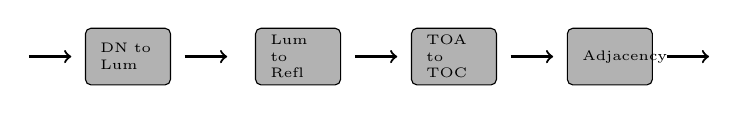
\begin{tikzpicture}[scale=0.18]
   \tiny

    \draw[->,thick] (0,0) --  +(3,0);
%     \pause

    \draw[fill=black!30,rounded corners=2pt] (4,-2) rectangle +(6,4);
    \node[text width= 0.7cm] (SensorModel) at (7,0) {DN to Lum};
%     \pause

    \draw[->,thick] (11,0) --  +(3,0);
%     \pause

    \draw[fill=black!30,rounded corners=2pt] (16,-2) rectangle +(6,4);
    \node[text width= 0.7cm] (SensorModel) at (19,0) {Lum to Refl};
%     \pause


    \draw[->,thick] (23,0) --  +(3,0);
%     \pause

    \draw[fill=black!30,rounded corners=2pt] (27,-2) rectangle +(6,4);
    \node[text width= 0.7cm] (SensorModel) at (30,0) {TOA to TOC};
%     \pause

    \draw[->,thick] (34,0) --  +(3,0);
%     \pause

    \draw[fill=black!30,rounded corners=2pt] (38,-2) rectangle +(6,4);
    \node[text width= 0.7cm] (SensorModel) at (41,0) {Adjacency};
%     \pause

    \draw[->,thick] (45,0) --  +(3,0);

 \end{tikzpicture}
\end{center}

  \begin{block}{Look like a pipeline}
  This is fully adapted to the pipeline architecture of OTB
  \end{block}

\end{frame}

\subsection[DN to lum]{Digital number to luminance}


\begin{frame}

  \frametitle{Digital number to luminance}
     \begin{columns}

   \column{0.7\textwidth}
  \begin{block}{Goal}
   \begin{itemize}
    \item Transform the digital number in the image into luminance
   \end{itemize}
  \end{block}
  Using the class otb::ImageToLuminanceImageFilter

  filterImageToLuminance->SetAlpha(alpha);

  filterImageToLuminance->SetBeta(beta);

  \column{0.3\textwidth}
  \footnotesize
  \begin{equation*}
   \mathbf{L_{TOA}^{k}} = \frac{ X^{k} } { \alpha_{k} } + \beta_{k}
  \end{equation*}
  \begin{itemize}
  \item $\mathbf{L_{TOA}^{k}}$ is the incident luminance (in
  $W.m^{-2}.sr^{-1}.\mu m^{-1}$)
  \item $\mathbf{X^{k}}$  digital number
  \item $\alpha_{k}$ absolute calibration gain for channel k
  \item $\beta_{k}$ absolute calibration bias for channel k
  \end{itemize}

  \end{columns}
\end{frame}

\begin{frame}[fragile]
  \frametitle{How to get these parameters?}
  \begin{block}{From metadata}
   \begin{itemize}
    \footnotesize
    \item Sometimes, the information can be present in the metadata but\ldots
    \item the specific format has to be supported (Spot, Quickbird,
          Ikonos are and more on the way)
   \end{itemize}
  \end{block}
  \begin{block}{From an ASCII file}
  \footnotesize
  \begin{verbatim}
  VectorType alpha(nbOfComponent);
  alpha.Fill(0);
  std::ifstream fin;
  fin.open(filename);
  double dalpha(0.);
  for( unsigned int i=0 ; i < nbOfComponent ; i++)
  {
      fin >> dalpha;
      alpha[i] = dalpha;
  }
  fin.close();
  \end{verbatim}
  \end{block}
\end{frame}

\subsection[lum to ref]{Luminance to reflectance}

\begin{frame}

  \frametitle{Luminance to reflectance}
     \begin{columns}

   \column{0.6\textwidth}
  \begin{block}{Goal}
   \begin{itemize}
    \item Transform the luminance into the reflectance
   \end{itemize}
  \end{block}
  \tiny
  Using the class otb::LuminanceToReflectanceImageFilter

  and setting parameters:

  \texttt{filterLumToRef-> SetZenithalSolarAngle(zenithSolar);}

  \texttt{filterLumToRef-> SetDay(day);}

  \texttt{filterLumToRef-> SetMonth(month);}

  \texttt{filterLumToRef-> SetSolarIllumination(solarIllumination);}

  \column{0.3\textwidth}
  \footnotesize
  \begin{equation*}
   \rho_{TOA}^{k} = \frac{ \pi.\mathbf{L_{TOA}^{k}} } { E_{S}^{k}.cos(\theta_{S}).d/d_{0} }
  \end{equation*}
  \begin{itemize}
\tiny
  \item $\mathbf{rho_{TOA}^{k}}$ reflectance
  \item $\theta_{S}$ zenithal solar angle
  \item $E_{S}^{k}$ solar illumination out of atmosphere at a distance 
  $d_{0}$ from the Earth
  \item $d/d_{0}$ ratio between Earth-Sun distance at 
  the acquisition and average Earth-Sun distance
  \end{itemize}

  \end{columns}
\end{frame}


\subsection{ToA to ToC}




\begin{frame}

  \frametitle{Top of atmosphere to top of canopy}

  \begin{block}{Goal}
   \begin{itemize}
    \item Compensate for the atmospheric effects
   \end{itemize}
  \end{block}
 
  
  \begin{columns}
  \column{0.5\textwidth}
  \footnotesize
  \begin{equation*}
   \rho_{S}^{unif} = \frac{ \mathbf{A} }{ 1 + Sx\mathbf{A} }
  \end{equation*}
  \column{0.5\textwidth}
  \begin{equation*}
   \mathbf{A} = \frac{ \rho_{TOA} - \rho_{atm} }{ T(\mu_{S}).T(\mu_{V}).t_{g}^{all gas} }
  \end{equation*}
  \end{columns}
  \begin{itemize}
  \item $\rho_{TOA}$ reflectance at the top of the atmosphere
  \item $\rho_{S}^{unif}$ ground reflectance under assumption
  of a lambertian surface and an uniform environment
  \item $\rho_{atm}$ intrinsic atmospheric reflectance
  \item $t_{g}^{all gas}$ spherical albedo of the atmosphere
  \item $T(\mu_{S})$ downward transmittance
  \item $T(\mu_{V})$ upward transmittance
  \end{itemize}
\end{frame}

\begin{frame}

  \frametitle{Top of Atmosphere to top of canopy}
  \begin{itemize}
  \tiny
  \item Using the class \texttt{otb::ReflectanceToSurfaceReflectanceImageFilter}

  \texttt{filterToAtoToC->SetAtmosphericRadiativeTerms(correctionParameters);}

  \item These parameters are filtered by the \texttt{otb::AtmosphericCorrectionParametersTo6SAtmosphericRadiativeTerms} from the \texttt{otb::AtmosphericCorrectionParameter} class 

\item this later class has the methods:

\texttt{parameters->SetSolarZenithalAngle();}

\texttt{parameters->SetSolarAzimutalAngle();}

\texttt{parameters->SetViewingZenithalAngle();}

\texttt{parameters->SetViewingAzimutalAngle();}

\texttt{parameters->SetMonth();}

\texttt{parameters->SetDay();}

\texttt{parameters->SetAtmosphericPressure();}

\texttt{parameters->SetWaterVaporAmount();}

\texttt{parameters->SetOzoneAmount();}

\texttt{parameters->SetAerosolModel();}

\texttt{parameters->SetAerosolOptical();}
\end{itemize}
\end{frame}


\subsection{Adjacency effects}


\begin{frame}

  \frametitle{Adjacency effects}
     \begin{columns}

   \column{0.6\textwidth}
  \begin{block}{Goal}
   \begin{itemize}
    \item Correct the adjacency effect on the radiometry of pixels
   \end{itemize}
  \end{block}

  \footnotesize
  Using the class \tiny \texttt{otb::SurfaceAdjacencyEffect6SCorrectionSchemeFilter}

  \footnotesize
  with the parameters

  \tiny 
  \texttt{filterAdjacency->SetAtmosphericRadiativeTerms();}

  \texttt{filterAdjacency->SetZenithalViewingAngle();}

  \texttt{filterAdjacency->SetWindowRadius();}

  \texttt{filterAdjacency->SetPixelSpacingInKilometers();}

  \column{0.4\textwidth}
  \footnotesize
  \begin{equation*}
  \rho{S} = \frac{ \rho_{S}^{unif}.T(\mu_{V}) - <\rho{S}>.t_{d}(\mu_{v}) }{ exp(-\delta/\mu_{v}) }
  \end{equation*}
  \begin{itemize}
    \item $\rho_{S}^{unif}$ ground reflectance assuming homogeneous environment
    \item $T(\mu_{V})$ upward transmittance
    \item $t_{d}(\mu_{S})$ upward diffuse transmittance
    \item $exp(-\delta/\mu_{v})$ upward direct transmittance
    \item $\rho{S}$ environment contribution to the pixel target reflectance in the total observed signal
  \end{itemize}

  \end{columns}
\end{frame}

\subsection{Hands On}


\begin{frame}
\frametitle{Hands On}
\begin{enumerate}
\item Monteverdi: Calibration $\rightarrow$ Optical calibration
\item Select the image to correct
\item Look at the parameters that are retrieved from the image metadata
\item Apply the correction
\item Look at the different levels
\end{enumerate}
\end{frame}

\section{Pansharpening}

\begin{frame}
  \frametitle{Pansharpening}
  \framesubtitle{Bring radiometric information to high resolution image}
\centering
\begin{columns}
\begin{column}{0.45\textwidth}
 \includegraphics[width=0.6\textwidth]{panSharp-pan-extract.jpg}\\
 \includegraphics[width=0.6\textwidth]{panSharp-xs-extract.jpg}
\end{column}
%\begin{column}{0.10\textwidth}
%$\Rightarrow$
%\end{column}
\begin{column}{0.45\textwidth}
 \includegraphics[width=0.6\textwidth]{panSharp-extract.jpg}
\end{column}
\end{columns}

\end{frame}

\begin{frame}
\frametitle{Hands On}
\begin{enumerate}
\item Monteverdi: Open two images, one PAN and one XS in the same geometry
\item Monteverdi: Filtering $\rightarrow$ Pan Sharpening
\end{enumerate}
\end{frame}

\end{document}
